\documentclass[smaller]{beamer}

\usepackage{iftex}

\RequireLuaTeX

\usepackage[]{fontspec}
\usepackage[brazilian]{babel}

\usepackage{dirtree}
\usepackage{tikz-qtree}
\usepackage{syntax}
\usepackage{pygmentex}
% \usepackage{jrmmisc}
\usepackage{tcolorbox}
\usepackage{relsize}
\usepackage{indentfirst}

% \setmainfont{Times New Roman}
% \setsansfont[Scale=MatchLowercase]{Helvetica}
% \setmonofont[Scale=MatchLowercase]{Courier}

% \setmainfont{Times New Roman}
% \setsansfont[Scale=MatchLowercase]{Helvetica LT Std}
% \setmonofont[Scale=MatchLowercase]{Courier Std}

% \setmainfont{DejaVu Serif}
% \setsansfont[Scale=MatchLowercase]{DejaVu Sans}
% \setmonofont[Scale=MatchLowercase]{DejaVu Sans Mono}

\setmainfont{Liberation Serif}
\setsansfont[Scale=MatchLowercase]{Liberation Sans}
\setmonofont[Scale=MatchLowercase]{Liberation Mono}

% \setmainfont{Lucida Std}
% \setsansfont[Scale=MatchLowercase]{Lucida Sans Std}
% \setmonofont[Scale=MatchLowercase]{Lucida Sans Typewriter Std}
% % \setmonofont[Scale=MatchLowercase]{Lucida Typewriter Std}

% \setmainfont{Luxi Serif}
% \setsansfont[Scale=MatchLowercase]{Luxi Sans}
% \setmonofont[Scale=MatchLowercase]{Luxi Mono}

% \setmainfont{Nimbus Roman No9 L}
% \setsansfont[Scale=MatchLowercase]{Nimbus Sans L}
% \setmonofont[Scale=MatchLowercase]{Nimbus Mono L}

% \setmainfont{Droid Serif}
% \setsansfont[Scale=MatchLowercase]{Droid Sans}
% \setmonofont[Scale=MatchLowercase]{Droid Sans Mono}	 % no bold

% \setmonofont[Scale=MatchLowercase]{Anonymous Pro}
% \setmonofont[Scale=MatchLowercase]{Consolas}
% \setmonofont[Scale=MatchLowercase]{Courier New}
% \setmonofont[Scale=MatchLowercase]{Cousine}
% \setmonofont[Scale=MatchLowercase]{DejaVu Sans Mono}
% \setmonofont[Scale=MatchLowercase]{Fantasque Sans Mono}
% \setmonofont[Scale=MatchLowercase]{Fira Code}
% \setmonofont[Scale=MatchLowercase]{Fira Mono}
% \setmonofont[Scale=MatchLowercase]{FreeMono}
% \setmonofont[Scale=MatchLowercase]{Hack}
% \setmonofont[Scale=MatchLowercase]{Input Mono Condensed}
% \setmonofont[Scale=MatchLowercase]{Iosevka Slab}
% \setmonofont[Scale=MatchLowercase]{Iosevka}
% \setmonofont[Scale=MatchLowercase]{Liberation Mono}
% \setmonofont[Scale=MatchLowercase]{Noto Mono}
% \setmonofont[Scale=MatchLowercase]{Source Code Pro}
% \setmonofont[Scale=MatchLowercase]{SF Mono}
% \setmonofont[Scale=MatchLowercase]{Ubuntu Mono}
\setmonofont[Scale=MatchLowercase]{M+ 1m}
% % 
% \setmonofont[Scale=MatchLowercase]{Letter Gothic Std}
% \setmonofont[Scale=MatchLowercase]{Lucida Sans Typewriter Std}
% \setmonofont[Scale=MatchLowercase]{Luxi Mono}


\setbeamercovered{transparent}
\hypersetup{colorlinks}
\usetheme{OuroPreto}

\newenvironment{tips}{%
  \textbf{Dicas:}\newline
  \begin{list}{*}{%
      \setlength{\topsep}{0pt}%
      \setlength{\itemsep}{0pt}%
      \setlength{\parsep}{0pt}%
    }%
  }{%
  \end{list}%
}

\usetikzlibrary{
  calc,
  shapes.multipart,
  chains,
  arrows,
  graphs,
  graphdrawing,
}

\usegdlibrary{
  layered
}

\tikzset{
  joined/.style = {
    join=by ->,
  },
  cons/.style = {
    draw,
    rounded corners,
    rectangle split,
    rectangle split parts=2,
    rectangle split horizontal,
    joined,
  },
  var/.style = {
    blue,
    joined,
  },
  null/.style = {
    fill,
    circle,
    inner sep=0mm,
    minimum size=2mm,
    joined,
  },
}

\renewcommand{\DTcomment}[1]{\textcolor{yellow}{\hrulefill}\sffamily\textcolor{blue}{#1}}
% \renewcommand\DTstylecomment{\sffamily\color{green}\textsc}
\renewcommand\DTstyle{\ttfamily\textcolor{red}}
\setlength{\DTbaselineskip}{12pt}
  
\newcommand{\semester}{2016.2}

\newcommand{\lang}{\textsl{EPLan}}


\setpygmented{lang=java,tabsize=3,sty=default}
\efboxsetup{hidealllines,backgroundcolor=yellow!28}

\mdfsetup{
  % backgroundcolor=green!10,
  roundcorner=2pt,
  skipabove=2pt,
  skipbelow=2pt,
  innerleftmargin=2pt,
  innerrightmargin=2pt,
  innertopmargin=.25\baselineskip,
  innerbottommargin=.25\baselineskip,
}


% syntax configuration
\renewcommand{\syntleft}{\normalfont\slshape\hspace{0.25em}}
\renewcommand{\syntright}{\hspace{0.25em}}
\renewcommand{\ulitleft}{\normalfont\ttfamily\bfseries\frenchspacing\color{red}\hspace{0.25em}}
\renewcommand{\ulitright}{\hspace{0.25em}}




\begin{document}

\title[compiler]{
  Compilador de \lang{}
}
\subject{Linguagens de Programação}
\author{José Romildo Malaquias}
\institute[UFOP]{
  Departamento de Computação\\
  Universidade Federal de Ouro Preto
}
\date{\semester}

\frame{\titlepage}

\frame{\tableofcontents}


\section{A estrutura do compilador}


\begin{frame}{Organização do compilador}
  \begin{itemize}
    \item Implementado na linguagem \textbf{Java}.
    \item Ferramentas auxiliares:
    \begin{itemize}
      \item \textbf{JFlex}: gerador de analisador léxico
      \item \textbf{CUP}: gerador de analisador sintático
      \item \textbf{LLVM}: gerador de código
      \item \textbf{Maven}: ferramenta de automação de compilação de
      projetos Java
    \end{itemize}
    \item Usa bibliotecas externas:
    \begin{itemize}
      \item \textbf{commons-lang3}: complementa as classes que estão
      em \pyginline|java.lang|.
      
      \item \textbf{jcommander}: framework Java muito pequeno que
      torna trivial a análise de parâmetros de linha de comando
      
      \item \textbf{javacpp-presets-llvm}: interface para a biblioteca
      LLVMC do projeto LLVM (infraestrutura de construçào de
      compilador escrita em C++)      
      
      \item \textbf{javaslang}: uma biblioteca funcional para Java 8+ que
      fornece tipos de dados persistentes e estruturas de controle
      funcionais

      \item \textbf{javaslang-render}: biblioteca de renderização para
      algumas estruturas de dados fornecidas por javaslang

      \item \textbf{junit}: \emph{framework} com suporte à criação de testes
      automatizados em Java

      \item \textbf{assertj}: fornece um rico conjunto de afirmações, com
      mensagens de erro úteis, melhorando a legibilidade dos testes
      automatizados em Java
    \end{itemize}
  \end{itemize}
\end{frame}

\begin{frame}[fragile]{Maven}
  \begin{itemize}
    \item Usado para automatizar a compilação de projetos.
    \item O projeto é configurado usando um \textbf{POM} (\emph{Project
      Object Model)}, que é armazenado em um arquivo \texttt{pom.xml}.
    \item O desenvolvimento pode ser feito em várias \textbf{fases},
    indicadas por \textbf{objetivos}, como:
    \begin{center}
      \begin{tabular}{ll}
        \textit{clean}                  & remover arquivos gerados    \\
        \textit{generate-sources}       & gerar código automático     \\
        \textit{process-resources}      & processar recursos          \\
        \textit{compile}                & compilar                    \\
        \textit{process-test-resources} & processar recursos de teste \\
        \textit{test-compile}           & testar compilação           \\
        \textit{test}                   & testar                      \\
        \textit{package}                & empacotar                   \\
        \textit{install}                & instalar                    \\
        \textit{deploy}                 & implantar
      \end{tabular}
    \end{center}
    \item Exemplo: compilar o projeto na linha de comando:
\begin{Verbatim}[frame=single]
$ mvn compile
\end{Verbatim}
  \end{itemize}
\end{frame}

\begin{frame}{Estrutura de diretórios do projeto}
  \small
  \noindent
    \dirtree{%
      .1 \lang{}-compiler.
      .2 src\DTcomment{código fonte do projeto}.
      .3 main\DTcomment{código fonte principal}.
      .4 c\DTcomment{código fonte em C}.
      .4 cup\DTcomment{código fonte para o CUP}.
      .4 java\DTcomment{código fonte em Java}.
      .4 jflex\DTcomment{código fonte para o JFlex}.
      .3 test\DTcomment{código fonte dos testes}.
      .4 java\DTcomment{código fonte dos testes em Java}.
      .2 target\DTcomment{arquivos gerados automaticamente}.
      .3 classes\DTcomment{classes geradas pelo compilador de Java}.
      .3 generated-sources\DTcomment{código fonte gerado por ferramentas}.
      .4 cup\DTcomment{código fonte gerado pelo CUP}.
      .4 jflex\DTcomment{código fonte gerado pelo JFlex}.
      .3 generated-test-sources\DTcomment{cód. fonte de testes gerado por ferramentas}.
      .3 test-classes\DTcomment{classes dos testes geradas pelo compilador de Java}.
      .2 pom.xml\DTcomment{arquivo de especificação do projeto}.
    }
\end{frame}

\section{Javaslang}

\begin{frame}[fragile,allowframebreaks]{Javaslang}
  \begin{itemize}
    \item Javaslang fornece várias estruturas de dados funcionais, como:
    \begin{itemize}
      \item tuplas
      \item listas
      \item árvores
      \begin{itemize}
        \item Árvores serão amplamente utilizadas para exibir as
        estruturas internas do compilador, incluindo as árvores
        sintáticas.
      \end{itemize}
    \end{itemize}
  \end{itemize}
\end{frame}
    
\begin{frame}[fragile,allowframebreaks]{\texttt{javaslang.Tuple2}}
  \footnotesize
\begin{pygmented}[]
import javaslang.Tuple;
import javaslang.Tuple2;

public class TestJavaslang {
  public static void main(String[] args) {
    Tuple2<String, Integer> person = Tuple.of("paul", 17);

    String name = person._1;
    Integer age = person._2;

    Tuple2<String, Integer> p =
            person.map(n -> n + " jones",
                       a -> a + 1);

    Tuple2<String, Integer> q =
            person.map((n, a) -> Tuple.of(n + " jones", a + 1));

    String s = person.transform((n, a) -> n + ": " + a);

    System.out.println(s);
  }
}
\end{pygmented}
\end{frame}



\begin{frame}[fragile,allowframebreaks]{\texttt{javaslang.collection.List}}
  \begin{itemize}
    \item Exemplos de listas (simplesmente) encadeadas:
\begin{pygmented}[]
List<Integer> list1 = List.empty();
List<String>  list2 = List.of("nice");
List<Integer> list3 = List.of(11, 12, 13);
List<Integer> list4 = list3.tail();
List<Integer> list5 = list4.prepend(10);
\end{pygmented}
    \begin{center}
      \begin{tikzpicture}[
        cons/.style={draw},
        var/.style={draw=none,blue},
        null/.style={circle,inner sep=0mm,minimum size=1mm},
        ]

        \graph [
        %layered layout,
        grow right sep,
        nodes={cons},
        ] {
          list1[var] -> n1[null,as={}];
          list2[var] -> nice -> n2[null,as={}];
          list3[var] -> 11 -> 12 -> 13 -> n3[null,as={}];
          list4[var] -> 12;
          list5[var] -> 10 -> 12;
        };

      \end{tikzpicture}
    \end{center}

    \framebreak
    
    \item Operando com cada elemento de uma lista:
\begin{pygmented}[]
List<Integer> lst = List.of(10, 20, 30);

for (Integer x : lst)
  System.out.println(x);

lst.forEach(x -> System.out.println(x));

lst.forEach(System.out::println);
\end{pygmented}

    \framebreak
    
    \item Aplicando uma função a cada elemento da lista e coletando os
    resultados em outra lista:
\begin{pygmented}[]
List<Double> a = List.of(4.0, 9.0, 25.0);
List<Double> c = a.map(Math::sqrt);
List<Double> b = a.map(x -> 2*x);
\end{pygmented}

    \framebreak
    
    \item Reduzindo uma lista:
\begin{pygmented}[]
List<String> a = List.of("1", "2", "3");
String str = a.fold("", (a1, a2) -> a1 + a2);

List<Integer> b = List.of(1, 2, 3, 4);
Integer sum = b.fold(0, (s, x) -> s + x);
\end{pygmented}

  \end{itemize}
\end{frame}



    
\begin{frame}[fragile,allowframebreaks]{\texttt{javaslang.collection.Tree}}
\begin{pygmented}[]
Tree<Integer> tree1 = Tree.empty();
Tree<String> tree2 = Tree.of("nice");
Tree<Integer> tree3 = Tree.of(99, 21, 22, 23);
Tree<Integer> tree4 = Tree.of(10,
                              Tree.of(5, Tree.of(2)),
                              Tree.of(7),
                              Tree.of(0),
                              Tree.of(19, Tree.of(3), Tree.of(8)));
\end{pygmented}
    \begin{center}
      \begin{tikzpicture}[
        cons/.style={draw},
        var/.style={draw=none,blue},
        null/.style={circle,inner sep=0mm,minimum size=1mm},
        ]

        \graph [
        layered layout,
        %grow right sep,
        nodes={cons},
        ] {
          tree1[var] -> n1[null,as={}];
          tree2[var] -> nice;
          tree3[var] -> 99 -> {21, 22, 23};
          tree4[var] -> 10 -> {5 -> 2, 7, 0, 19 -> {3, 8}};
        };

      \end{tikzpicture}
    \end{center}
\end{frame}


\begin{frame}[fragile,allowframebreaks]{\texttt{javaslang.render.text.PrettyPrinter}}
  \small
  \begin{columns}[t]
    \begin{column}{.75\textwidth}
\begin{pygmented}[]
import javaslang.collection.Tree;

import javaslang.render.text.PrettyPrinter;

final Tree<String> tree =
       Tree.of("Ann",
               Tree.of("Mary",
                       Tree.of("John",
                               Tree.of("Avila")),
                       Tree.of("Karen",
                               Tree.of("Frank")),
                       Tree.of("Steven\nAbbot\nBraddock")),
               Tree.of("Peter",
                       Tree.of("Paul\nPalucci"),
                       Tree.of("Anthony")),
               Tree.of("Christopher",
                       Tree.of("Samuel")));

final String out = PrettyPrinter.pp(tree);
\end{pygmented}
    \end{column}
    \begin{column}{.25\textwidth}
\begin{Verbatim}
Ann
├──Mary
│  ├──John
│  │  └──Avila
│  ├──Karen
│  │  └──Frank
│  └──Steven
│     Abbot
│     Braddock
├──Peter
│  ├──Paul
│  │  Palucci
│  └──Anthony
└──Christopher
   └──Samuel
\end{Verbatim}
    \end{column}
  \end{columns}
\end{frame}

\begin{frame}[fragile,allowframebreaks]{\texttt{javaslang.render.text.Boxes}}
  \footnotesize
\begin{pygmented}[]
import javaslang.collection.Tree;
import javaslang.render.text.Boxes;

final Tree<String> tree = /* ... */

final String out = Boxes.box(tree).toString();
\end{pygmented}

\begin{verbatim}
                           ┌───┐                            
                           │Ann│                            
                           └─┬─┘                            
             ┌───────────────┴──────┬────────────────┐      
          ┌──┴─┐                 ┌──┴──┐       ┌─────┴─────┐
          │Mary│                 │Peter│       │Christopher│
          └──┬─┘                 └──┬──┘       └─────┬─────┘
   ┌───────┬─┴───────┐         ┌────┴────┐           │      
┌──┴─┐  ┌──┴──┐ ┌────┴───┐ ┌───┴───┐ ┌───┴───┐   ┌───┴──┐   
│John│  │Karen│ │ Steven │ │ Paul  │ │Anthony│   │Samuel│   
└──┬─┘  └──┬──┘ │ Abbot  │ │Palucci│ └───────┘   └──────┘   
   │       │    │Braddock│ └───────┘                        
┌──┴──┐ ┌──┴──┐ └────────┘                                  
│Avila│ │Frank│                                             
└─────┘ └─────┘                                             
\end{verbatim}
\end{frame}


\begin{frame}[fragile,allowframebreaks]{\texttt{javaslang.render.text.DotFile}}
  \small
  \begin{columns}[t]
    \begin{column}{.5\textwidth}
\begin{pygmented}[]
import javaslang.collection.Tree;
import javaslang.render.dot.DotFile;

final Tree<String> tree = /* ... */;

DotFile.write(tree, "tree.dot");
\end{pygmented}
    \end{column}
    \begin{column}{.5\textwidth}
      \begin{itemize}
        \item Dot é uma linguagem para descrever grafos.
        \item É necessário o pacote \textbf{graphviz}.
      \end{itemize}
\begin{Verbatim}[frame=single]
$ dot -Tpng -O tree.dot
\end{Verbatim}
    \end{column}
  \end{columns}
  \begin{center}
    \makebox[0pt][r]{\texttt{tree.dot.png}}
    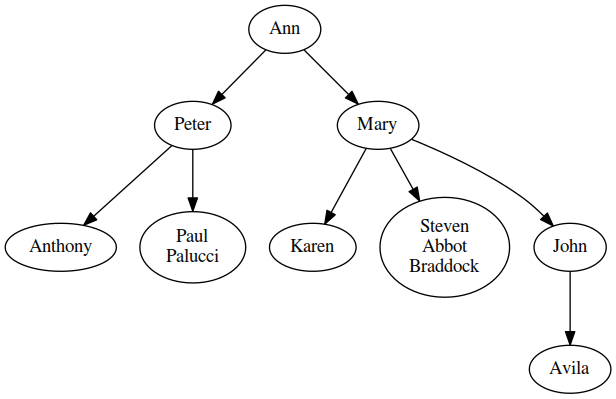
\includegraphics[scale=.35]{images/tree.png}
  \end{center}
\end{frame}

\section{Posição no código fonte}

\begin{frame}[fragile,allowframebreaks]{Localização no código fonte}
  \begin{itemize}
    \item A localização é usada para reportar erros.
    \item Indica onde uma frase do programa começa e termina no código
    fonte.
    \item Representada pela classe \pyginline|parse.Loc|
    \begin{pygmented}[lang=java]
Loc(Location left, Location right)
    \end{pygmented}
    \item Usa o tipo
    \begin{pygmented}[lang=java]
java_cup.runtime.ComplexSymbolFactory.Location
    \end{pygmented}
    contendo informações como:
    \begin{itemize}
      \item nome da unidade de compilação (arquivo fonte)
      \item número da linha
      \item número da coluna
    \end{itemize}
  \end{itemize}
\end{frame}

\begin{frame}[fragile,allowframebreaks]{Construção da localização}
  \begin{itemize}
    \item Alguns métodos de fábrica:
\begin{pygmented}[]
import java_cup.runtime.Symbol;
import java_cup.runtime.ComplexSymbolFactory.ComplexSymbol;
import java_cup.runtime.ComplexSymbolFactory.Location;

/* ... */

public static Loc loc()
public static Loc loc(Location left)
public static Loc loc(Location left, Location right)
public static Loc loc(Symbol symbol)
public static Loc loc(Symbol a, Symbol b)
public static Loc loc(ComplexSymbol symbol)
public static Loc loc(ComplexSymbol a, ComplexSymbol b)
\end{pygmented}
    
    \item \pyginline|Symbol| e \pyginline|ComplexSymbol| representam
    símbolos terminais
  \end{itemize}
\end{frame}


\section{Gerenciamento de erros}

\begin{frame}[fragile,allowframebreaks]{Reportagem de erro}
  \begin{itemize}
    \item Os erros são reportados por meio do mecanismo de
    \textbf{exceções} de Java.
    \item Erros no programa fonte são representados pela classe
    \pyginline|error.CompileError|, subclasse de
    \pyginline|RuntimeError|.
    \item Erros na implementação do compilador são representados pela
    classe \pyginline|error.FatalError|, também subclasse de
    \pyginline|RuntimeError|.
    \item A classe \pyginline|error.ErrorHelper| tem alguns métodos
    estáticos que facilitam a criação de objetos de erro:
\begin{pygmented}[]
static CompilerError error(String message)
static CompilerError error(String format, Object... args)
static CompilerError error(Loc loc, String format, Object... args)

static FatalError fatal(String format, Object... args)
\end{pygmented}
  \end{itemize}
\end{frame}


\section{Análise léxica}

\begin{frame}[fragile,allowframebreaks]{Símbolos terminais}
  \begin{itemize}
    \item Os \textbf{símbolos terminais} são definidos na gramática
    livre de contexto do CUP (arquivo
    \texttt{src/main/cup/parser.cup}).
    \item Exemplos:
\begin{pygmented}[]
terminal String LITREAL;
terminal        PLUS, MINUS, TIMES, DIV;
terminal        LPAREN, RPAREN;
\end{pygmented}
    
    \item O CUP gera uma interface \pyginline|parse.SymbolConstants|
    contendo a definição de constantes correspondentes aos terminais
    que foram declarados.
    
    \item Quando relevante os terminais podem ter um valor semântico
    associado.

    \item A classe \pyginline|ComplexSymbol| é usada para representar
    os símbolos terminais, contendo as seguintes informações:
    \begin{itemize}
      \item classificação (como declarado na gramática)
      \item lexema
      \item localização (começo e fim) no código fonte
      \item valor semântico
    \end{itemize}
  \end{itemize}
\end{frame}

\begin{frame}[fragile,allowframebreaks]{Regras léxicas}
  \begin{itemize}
    \item O analisador léxico é gerado pelo \textbf{JFlex}.
    \item As regras léxicas são especificadas no arquivo
    \alert{\texttt{src/main/jflex/lexer.jflex}}.
    \item O JFlex cria a classe \pyginline|parse.Lexer| compatível com
    o CUP.
    \item Os \textbf{lexemas} (palavras que formam os símbolos
    léxicos) são descritos por \textbf{expressões regulares}.
    \item A classificação so símbolo terminal é feita na \textbf{ação
      semântica} (código em Java que faz parte da regra léxica).
    \item Para facilitar a criação dos diversos símbolos léxicos
    recomenda-se o uso dos \alert{métodos auxiliares} (definidos no
    próprio arquivo de especificação):
\begin{pygmented}[]
private Symbol tok(int type, String lexeme, Object value)
private Symbol tok(int type, Object value)
private Symbol tok(int type)
\end{pygmented}
  \end{itemize}
\end{frame}


\begin{frame}[fragile,allowframebreaks]{Exemplo de regras léxicas}
\begin{pygmented}[lang=text]
[ \t\f\n\r]+           { /* skip */ }

[0-9]+ ("." [0-9]+)?   { return tok(LITREAL, yytext()); }

"+"                    { return tok(PLUS); }
"-"                    { return tok(MINUS); }
"*"                    { return tok(TIMES); }
"/"                    { return tok(DIV); }
"("                    { return tok(LPAREN); }
")"                    { return tok(RPAREN); }

.                      { throw error(Loc.loc(locLeft()),
                                     "unexpected char '%s'",
                                     yytext()); }
\end{pygmented}
\end{frame}


\section{Análise sintática}

\begin{frame}[fragile,allowframebreaks]{Análise sintática}
  \begin{itemize}
    \item A especificação sintática (\textbf{gramática livre de
      contexto}) é feita no arquivo
    \alert{\texttt{src/main/cup/parser.cup}}.
    \item Algumas opções de execução do CUP são indicadas no arquivo
    \alert{\texttt{pom.xml}}.
    \item O analisador sintático é gerado pelo \textbf{CUP}, que cria
    a classe \pyginline|parse.Parser| e a interface
    \pyginline|parse.SymbolConstants|.
    \item Na gramática livre de contexto são especificados:
    \begin{itemize}
      \item os símbolos terminais
      \item os símbols não terminais
      \item o símbolo inicial
      \item as regras de produção
    \end{itemize}
  \end{itemize}
\end{frame}

\begin{frame}[fragile,allowframebreaks]{Ações semânticas}
  \begin{itemize}
    \item Quando um símbolo (terminal ou não terminal) tem um
    \textbf{valor semântico}, o tipo do valor semântico é informado na
    declaração do símbolo.
    \item O cálculo do valor semântico do símbolo no lado esquerdo de
    uma regra de produção é feito usando os valores semênticas dos
    símbolos que aparecem no lado direiro da regra através de uma
    \textbf{ação semântica} (código em Java).
    \item Quando um \alert{nome} é associado a um símbolo no lado
    direito de uma regra (por exemplo \pyginline|exp:nome|), o CUP
    cria três variáveis (no exemplo \pyginline|nome|,
    \pyginline|nomexleft| e \pyginline|nomexright|) no codigo gerado,
    contendo o valor semântico, a localização esquerda (onde começa no
    código fonte), e a localização direita (onde termina no código
    fonte) do símbolo, respectivamente.
  \end{itemize}
\end{frame}


\begin{frame}[fragile,allowframebreaks]{Exemplo de gramática para o CUP}
  \scriptsize
\begin{pygmented}[]
terminal String LITREAL;
terminal        PLUS, MINUS, TIMES, DIV;
terminal        LPAREN, RPAREN;

non terminal Exp exp;
non terminal Exp term;
non terminal Exp factor;

start with exp;

exp ::=
  exp:x PLUS term:y      {: RESULT = new ExpBinOp(ExpBinOp.Op.PLUS, x, y);  :}
| exp:x MINUS term:y     {: RESULT = new ExpBinOp(ExpBinOp.Op.MINUS, x, y); :}
| term:x                 {: RESULT = x;                                     :}
;

term ::=
| term:x TIMES factor:y  {: RESULT = new ExpBinOp(ExpBinOp.Op.TIMES, x, y); :}
| term:x DIV factor:y    {: RESULT = new ExpBinOp(ExpBinOp.Op.DIV, x, y);   :}
| factor:x               {: RESULT = x;                                     :}
;

factor ::=
  LITREAL:x              {: RESULT = new ExpReal(x);                        :}
| LPAREN exp:x RPAREN    {: RESULT = x;                                     :}
;
\end{pygmented}
\end{frame}


\section{Árvores sintáticas}

\begin{frame}[fragile,allowframebreaks]{Árvores sintáticas}
  \begin{itemize}
    \item \textbf{Árvore sintática} é uma \alert{estrutura de dados
      hierárquica} que representa a estrutura sintática do programa
    fonte.
    \item A \textbf{raiz} da árvore é o \alert{símbolo inicial} da
    gramática.
    \item As \textbf{folhas} são os \alert{símbolos terminais} que,
    lidos da esquerda para a direita, correspondem ao programa fonte.
    \item Pode ser:
    \begin{itemize}
      \item \textbf{concreta}: todos os símbolos na sequência de
      derivação são colocados na árvore
      \item \textbf{abstrata}: apenas as informações relevantes para o
      entendimento da estrutura do programa são mantidos na árvore
    \end{itemize}
    \item A saída do \textbf{analisador sintático} é uma árvore
    sintática abstrata (\alert{AST}).
  \end{itemize}
\end{frame}

\begin{frame}[fragile,allowframebreaks]{Representação}
  \begin{itemize}
    \item A representação das árvores sintáticas é feita através de
    classes no pacote \pyginline|absyn|.
    \item A classe abstrata \pyginline|absyn.AST| é superclasse de
    todas as árvores sintáticas abstratas.
    \item Esta classe implementa a interface \pyginline|ToTree|:
\begin{pygmented}[]
package javaslang.render;

import javaslang.collection.Tree;

public interface ToTree<E> {
    public abstract Tree.Node<E> toTree();
}
\end{pygmented}
    \item O método \pyginline|toTree| converte a árvore abstrata em
    uma estrutura de dados geral para árvores cujos nós armazenam
    strings, útil na apresentação visual da árvore sintática.
  \end{itemize}
\end{frame}


\begin{frame}[fragile,allowframebreaks]{Definindo as árvores abstratas}
  \begin{itemize}
    \item Para cada \alert{categoria sintática} (como expressões,
    comandos, ou declarações) reprentada por um \textbf{símbolo não
      terminal} definimos uma subclasse abstrata de
    \pyginline|absyn.AST|.
    \item Para cada \alert{forma} da categoria sintática para um não
    terminal (como as formas de expressão: expressão constante,
    operação binária, chamada de função, etc.), representada por uma
    \textbf{regra de produção}, definamos uma subclasse da classe que
    representa aquela forma específica da categoria sintática.
    \item 
    Nesta classe deve-se:
    \begin{itemize}
      \item definir os \alert{campos} necessários para os componentes
      (sub-árvores) da árvore sintática,
      \item definir \alert{construtores} que inicializam estes campos
      com valores passados como argumentos,
      \item definir o método \pyginline|toTree|.
    \end{itemize}
  \end{itemize}
\end{frame}

\begin{frame}[fragile,allowframebreaks]{A classe AST}
\begin{pygmented}[]
package absyn;

import javaslang.render.ToTree;
import org.apache.commons.lang3.builder.ToStringBuilder;
import org.apache.commons.lang3.builder.ToStringStyle;

public abstract class AST implements ToTree<String> {

   @Override
   public String toString() {
      return ToStringBuilder.reflectionToString(
                 this,
                 ToStringStyle.SHORT_PREFIX_STYLE);
   }

}
\end{pygmented}
\end{frame}

\begin{frame}[fragile,allowframebreaks]{A classe Exp}
\begin{pygmented}[]
package absyn;

public abstract class Exp extends AST {
}
\end{pygmented}
\end{frame}

\begin{frame}[fragile,allowframebreaks]{A classe ExpReal}
\begin{pygmented}[]
package absyn;

import javaslang.collection.Tree;

public class ExpReal extends Exp {

   public final String value;

   public ExpReal(String value) {
      this.value = value;
   }

   @Override
   public Tree.Node<String> toTree() {
      return Tree.of("ExpReal: " + value);
   }
}
\end{pygmented}
\end{frame}

\begin{frame}[fragile,allowframebreaks]{A classe ExpReal}
  \relscale{0.78}
\begin{pygmented}[]
package absyn;

import javaslang.collection.Tree;

public class ExpBinOp extends Exp {

   public enum Op {PLUS, MINUS, TIMES, DIV}

   public final Op op;
   public final Exp left;
   public final Exp right;

   public ExpBinOp(Op op, Exp left, Exp right) {
      this.op = op;
      this.left = left;
      this.right = right;
   }

   @Override
   public Tree.Node<String> toTree() {
      return Tree.of("ExpBinOp: " + op, left.toTree(), right.toTree());
   }
}
\end{pygmented}
\end{frame}


\section{Geração de código}

\begin{frame}[fragile,allowframebreaks]{Representação intermediária}
  \begin{itemize}
    \item A árvore sintática do programa fonte é traduzida para uma
    representação intermediária do código fonte.
    \item Usaremos a representação intermediária do framework
    \textbf{LLVM}.
    \item A biblioteca Java \texttt{javacpp-presets-llvm} será usada
    para criar a representação intermediária.
    \item A classe \pyginline|absyn.Exp| deve ter um método abstrato
    para converter uma expressão para a sua representação
    intermediária.
\begin{pygmented}[]
import static org.bytedeco.javacpp.LLVM.*;
/* ... */
public abstract LLVMValueRef translate(LLVMModuleRef module,
                                       LLVMBuilderRef builder);
\end{pygmented}
    \item Suas subclasses devem implementar este método.
  \end{itemize}
\end{frame}

\begin{frame}[fragile,allowframebreaks]{Representação intermediária de constantes}
\begin{pygmented}[]
package absyn;

// ...
import static org.bytedeco.javacpp.LLVM.*;

public class ExpReal extends Exp {
   // ...

   @Override
   public LLVMValueRef translate(LLVMModuleRef module,
                                 LLVMBuilderRef builder) {
      return LLVMConstRealOfString(LLVMDoubleType(), value);
   }
}
\end{pygmented}
\end{frame}

\begin{frame}[fragile,allowframebreaks]{Representação intermediária de operação binária}
  \relscale{0.76}
\begin{pygmented}[]
package absyn;

// ...
import static org.bytedeco.javacpp.LLVM.*;
import static error.ErrorHelper.fatal;

public class ExpBinOp extends Exp {
   // ...

   @Override
   public LLVMValueRef translate(LLVMModuleRef module, LLVMBuilderRef builder) {
      final LLVMValueRef v_left = left.translate(module, builder);
      final LLVMValueRef v_right = right.translate(module, builder);
      switch (op) {
         case PLUS:  return LLVMBuildFAdd(builder, v_left, v_right, "addtmp");
         case MINUS: return LLVMBuildFSub(builder, v_left, v_right, "subtmp");
         case TIMES: return LLVMBuildFMul(builder, v_left, v_right, "multmp");
         case DIV:   return LLVMBuildFDiv(builder, v_left, v_right, "divtmp");
         default:    fatal("unknown operator %s in binary operation", op);
                     return LLVMConstReal(LLVMDoubleType(), 0);
      }
   }
}
\end{pygmented}
\end{frame}



\begin{frame}[fragile,allowframebreaks]{Atividade 1}
  \begin{tcolorbox}[title=Inverso aditivo]
    Implementar a operação que calcula o inverso aditivo (ou negação)
    à linguagem \lang{}. Será usado o operador unário prefixo
    \pyginline|-|, com precedência maior que dos operadores
    aritméticos binários.
    \begin{enumerate}
      \item Definir uma nova classe \pyginline|absyn.ExpNegate|
      \begin{itemize}
        \item subclasse de \pyginline|absyn.Exp|
        \item contendo um campo correspondente ao operando da negação
        \item implementar o método \pyginline|toTree|
        \item implementar o método \pyginline|translate|
      \end{itemize}
      \item Acrescentar uma regra de produção adequada na gramática da
      linguagem.
    \end{enumerate}

    \begin{tips}
      \item Na geração de código use o método

      \href{http://bytedeco.org/javacpp-presets/llvm/apidocs/org/bytedeco/javacpp/LLVM.html#LLVMBuildFNeg-org.bytedeco.javacpp.LLVM.LLVMBuilderRef-org.bytedeco.javacpp.LLVM.LLVMValueRef-java.lang.String-}{\pyginline|LLVMBuildFNeg|}

      \href{http://llvm.org/docs/doxygen/html/group__LLVMCCoreInstructionBuilder.html#gaf748025627b03f4f2659b006b127b758}{\pyginline|LLVMBuildFNeg|}
    \end{tips}
\end{tcolorbox}

  \framebreak
  
  Comandos úteis:
\begin{Verbatim}[frame=single]
$ cd <working directory>/eplan
$ git checkout master
$ git pull upstream master
$ git checkout -b atividade1
$ # desenvolva sua atividade
$ # faça testes
$ git status
$ git add <arquivos modificados>
$ git commit -m <mensagem>
$ git push origin atividade1
$ # faça um pull request no github
\end{Verbatim}
\end{frame}


\section{Análise semântica}

\begin{frame}[fragile,allowframebreaks]{Anotando a localização na árvore sintática}
  \begin{itemize}
    \item Na análise semêntica os erros encontrados devem ser
    reportados.

    \item Deve-se indicar a localização do erro no código fonte.

    \item Por isto a árvore sintática deve conter a
    \textbf{localização}.

    \item O atributo \pyginline|loc| foi adicionado à classe abstrata
    \pyginline|absyn.AST|.
\begin{pygmented}[]
import parse.Loc;

public abstract class AST implements ToTree<String> {

   // Location where the phrase was found in the source code
   protected final Loc loc;

   public AST(Loc loc) {
      this.loc = loc;
   }

   // ...
}
\end{pygmented}

    \framebreak
    
    \item Um argumento correspondente foi adicionado aos construtores
    das subclasses de \pyginline|absyn.AST|. Por exemplo:
\begin{pygmented}[]
public class ExpReal extends Exp {

   public final String value;

   public ExpReal(Loc loc, String value) {
      super(loc);
      this.value = value;
   }

   // ...
}
\end{pygmented}

    \framebreak

    \item A criação das árvores sintáticas nas ações semânticas do
    analisador sintático deve informar a localização. Exemplo:
\begin{pygmented}[]
factor ::=
  LITREAL:x {: RESULT = new ExpReal(loc(xxleft,xxright), x); :}
;
\end{pygmented}

    \item Na regra de produção, ao indicarmos o nome do valor
    semântico de um símbolo, são criadas três variáveis no analisador
    gerado pelo CUP, contendo as seguintes informações:
    \begin{itemize}
      \item valor semântico do símbolo
      \item posição onde o símbolo começou no código fonte
      \item posição onde o símbolo terminou no código fonte
    \end{itemize}
    No exemplo estas variáveis são respectivamente \pyginline|x|,
    \pyginline|xxleft|, e \pyginline|xxright|.
  \end{itemize}
\end{frame}


\begin{frame}[fragile,allowframebreaks]{Representando os tipos da linguagem}
  \begin{itemize}
    \item O pacote \pyginline|type| contém classes usadas para representar
    os tipos da linguagem sendo compilada.
    \item A representação geral é \pyginline|Type|.
    \item \pyginline|Type| é uma classe abstrata, com subclasses concretas
    para representar cada uma das possibiliades:
    \begin{center}
      \small
      \begin{tabular}{lll} \hline
        \textbf{descrição}   & \textbf{classe}    & \textbf{objeto}                                          \\\hline
        \texttt{bool}        & \pyginline|BOOL|   & \pyginline|BOOL.T|                                       \\
        \texttt{int}         & \pyginline|INT|    & \pyginline|INT.T|                                        \\
        \texttt{real}        & \pyginline|REAL|   & \pyginline|REAL.T|                                       \\
        \texttt{char}        & \pyginline|CHAR|   & \pyginline|CHAR.T|                                       \\
        \texttt{string}      & \pyginline|STRING| & \pyginline|STRING.T|                                     \\
        \emph{array}         & \pyginline|ARRAY|  & \pyginline|new Array(Type element)|                      \\
        \emph{registro}      & \pyginline|RECORD| & \pyginline|new RECORD(List<Tuple2<Symbol,Type>> fields)| \\
        \emph{registro nulo} & \pyginline|NIL|    & \pyginline|NIL.T|                                        \\
        \texttt{unit}        & \pyginline|UNIT|   & \pyginline|UNIT.T|                                       \\
        \emph{nome}          & \pyginline|NAME|   & \pyginline|new Name(Symbol name, Type binding)|          \\\hline
      \end{tabular}
    \end{center}
  \end{itemize}    
\end{frame}

\begin{frame}[fragile,allowframebreaks]{Algumas operações com tipos}
  \begin{description}
    \item[\pyginline|Type actual()|]\mbox{}\newline
    \begin{itemize}
      \item Retorna a representação que é de fato usada para o tipo.
      \item É o próprio objeto, exceto para a classe \pyginline|NAME|, onde
      é retornado \pyginline|binding.actual()|.
    \end{itemize}
    \framebreak
    
    \item[\pyginline|boolean is(Type type)|]\mbox{}\newline
    \begin{itemize}
      \item Verifica se o tipo que recebe a mensagem é compatível (é igual
      ou pode ser convertido para) o tipo dado como argumento.
      \item Retorna \pyginline|true| somente se os dois tipos forem
      idênticos, exceto nos seguintes casos:
      \begin{itemize}
        \item o tipo do registo nulo (\texttt{nil}), \pyginline|NIL|, é
        compatível com \pyginline|NIL| e com qualquer tipo registro,
        \item um tipo \pyginline|NAME| é compatível com algum tipo, se
        e somente se o seu atributo \pyginline|binding| for compatível
        com o tipo.
      \end{itemize}
    \end{itemize}
    \framebreak

    \item[\pyginline|boolean is(Type... types)|]\mbox{}\newline
    \begin{itemize}
      \item Verifica a compatibilidade com algum dos tipos dados como
      argumentos.
    \end{itemize}
  \end{description}
\end{frame}


\begin{frame}[fragile,allowframebreaks]{Reportando erros comuns}
  \begin{itemize}
    \item A interface \pyginline|semantic.SemanticHelper| define
    alguns métodos para reportar erros comumente encontrados pelo
    compilador no código fonte.

    \item Um dos erros mais comuns é a inconsistência de tipos.
\begin{pygmented}[]
public interface SemanticHelper {

   static CompilerError typeMismatch(Loc loc, Type found, Type... expected)
      // ...
   }

   // ...
}
\end{pygmented}
  \end{itemize}
\end{frame}

\begin{frame}[fragile,allowframebreaks]{Análise semântica}
  \begin{itemize}
    \item O analisador semântico
    \begin{itemize}
      \item verifica a consistência do programa
      \item calcula o tipo das expressões
    \end{itemize}
    \item Expressões tem um atributo \pyginline|type| cujo valor é a
    representação do tipo obtido para a expressão.
    \item \pyginline|type| é calculado pelo analisador semântico.
\begin{pygmented}[]
import types.Type;

public abstract class Exp extends AST {

   // Type of the expression, calculated by the semantic analyser
   public Type type;

   // Obtain the type of the expression as a string prefixed by the given text.
   protected String annotateType(String text) {
      final String theType = type == null ? "" : "\n<" + type + ">";
      return text + theType;
   }

   // ...
}
\end{pygmented}

    \framebreak
    
    \item O método \pyginline|semantic| da classe
    \pyginline|absyn.Exp| faz análise semântica da expressão.
    \begin{itemize}
      \item Usa o método auxiliar \pyginline|semantic_| para fazer a
      análise semântica de fato, obtendo o tipo da expressão.
      \item Coloca o tipo encontrado no atributo \pyginline|type|.
    \end{itemize}
\begin{pygmented}[]
public abstract class Exp extends AST {
   // ...

   // Do semantic analysis of the expression
   public Type semantic() {
      type = semantic_();
      return type;
   }

   // Type check the expression. Should be defined in the concrete subclasses.
   protected abstract Type semantic_();
}
\end{pygmented}
    
    \item Subclasses de \pyginline|absyn.Exp| devem definir o método
    \pyginline|semantic_| apropriadamente.
    
    \item Por exemplo:
\begin{pygmented}[]
public class ExpReal extends Exp {
   // ...

   @Override
   protected Type semantic_() {
      return REAL.T;
   }
}
\end{pygmented}

  \end{itemize}
\end{frame}



\begin{frame}[fragile,allowframebreaks]{Atividade 2: literal inteiro}
  Implementar \textbf{literais inteiros} no compilador de \lang{}.
  \begin{enumerate}
    \item Para desenvolver esta atividade faça o \emph{checkout} da
    \alert{versão 0.17} do projeto.
    
    \item Definir uma nova classe \pyginline|types.INT| para
    representar o tipo \texttt{int} de \lang{}.

    \item Definir uma nova classe \pyginline|absyn.ExpInt| para
    representar as árvores sintáticas das constantes inteiras:
    \begin{itemize}
      \item subclasse de \pyginline|absyn.Exp|
      \item contendo um campo correspondente ao valor da constante
      \item implementar o método \pyginline|toTree|
      \item implementar o método \pyginline|semantic_|
      \item implementar o método \pyginline|translate|
    \end{itemize}
    
    \item Modifique a classe \pyginline|absyn.ExpBinOp| de forma que
    os operadores aritméticos aceitem operandos inteiros e
    reais. Neste momento não é necessário fazer conversão implícita
    dos operandos de inteiro para real. Por hora os operandos devem
    apenas ser do mesmo tipo numérico.

    \item Acrescentar na gramática da linguagem:
    \begin{itemize}
      \item o símbolo terminal \pyginline|LITINT|
      \item uma regra de produção adequada
    \end{itemize}

    \item Na especificação léxica da linguagem
    \begin{itemize}
      \item acrescentar uma regra para o literal inteiro:

      Um literal inteiro é uma sequência não vazia de dígitos
      decimais.

      \item modificar a regra do literal real para não casar com
      literais inteiros
    \end{itemize}

    \item Definir a função \pyginline|__eplan_print_int| (em C) na
    biblioteca padrão de \lang{} para exibir um valor inteiro. O
    protótipo da função deve ser:
\begin{pygmented}[]
extern void __eplan_print_int(const int32_t x)
\end{pygmented}
    O tipo \pyginline|int32_t| está definido em
    \texttt{inttypes.h}. Use a função \pyginline|printf| e a macro
    \pyginline|PRIi32| na formatação da saída.

    \item Modificar o método \pyginline|addRuntime| na classe
    \pyginline|translate.Generator| para adicionar o protótipo da função
    \pyginline|__eplan_print_int| no código gerado.
    
    \item Modificar o método \pyginline|addPrintResult| na classe
    \pyginline|codegen.Generator| para considerar o caso de valores
    inteiros. Este método gera código para exibir o valor de uma
    expressão na saída padrão.
  \end{enumerate}

  \begin{tips}
    \item Na geração de código use os métodos

    \href{http://bytedeco.org/javacpp-presets/llvm/apidocs/org/bytedeco/javacpp/LLVM.html#LLVMConstIntOfString-org.bytedeco.javacpp.LLVM.LLVMTypeRef-java.lang.String-byte-}{\pyginline|LLVMConstIntOfString|}

    \href{http://bytedeco.org/javacpp-presets/llvm/apidocs/org/bytedeco/javacpp/LLVM.html#LLVMBuildAdd-org.bytedeco.javacpp.LLVM.LLVMBuilderRef-org.bytedeco.javacpp.LLVM.LLVMValueRef-org.bytedeco.javacpp.LLVM.LLVMValueRef-java.lang.String-}{\pyginline|LLVMBuildAdd|}

    \href{http://bytedeco.org/javacpp-presets/llvm/apidocs/org/bytedeco/javacpp/LLVM.html#LLVMBuildSub-org.bytedeco.javacpp.LLVM.LLVMBuilderRef-org.bytedeco.javacpp.LLVM.LLVMValueRef-org.bytedeco.javacpp.LLVM.LLVMValueRef-java.lang.String-}{\pyginline|LLVMBuildSub|}

    \href{http://bytedeco.org/javacpp-presets/llvm/apidocs/org/bytedeco/javacpp/LLVM.html#LLVMBuildMul-org.bytedeco.javacpp.LLVM.LLVMBuilderRef-org.bytedeco.javacpp.LLVM.LLVMValueRef-org.bytedeco.javacpp.LLVM.LLVMValueRef-java.lang.String-}{\pyginline|LLVMBuildMul|}

    \href{http://bytedeco.org/javacpp-presets/llvm/apidocs/org/bytedeco/javacpp/LLVM.html#LLVMBuildSDiv-org.bytedeco.javacpp.LLVM.LLVMBuilderRef-org.bytedeco.javacpp.LLVM.LLVMValueRef-org.bytedeco.javacpp.LLVM.LLVMValueRef-java.lang.String-}{\pyginline|LLVMBuildSDiv|}
\end{tips}
\end{frame}



% \section{Identificadores}


% \begin{frame}[fragile,allowframebreaks]{Representando identificadores}
%   \begin{itemize}
%     \item \textbf{Identificadores} são nomes dados a diversas entidades em
%     um programa: tipos, variáveis, funções, módulos, classes, etc.
%     \item Quando uma declaração é analisada, alguma informação sobre o
%     identificador é armazenada em um \textbf{ambiente} (um dicionário,
%     também chamado de \textbf{tabela de símbolos}), contendo por exemplo:
%     \begin{itemize}
%       \item tipo de uma variável
%       \item tipo dos argumentos e do resultado de uma função
%       \item estrutura de um tipo
%     \end{itemize}
%     \item Posteriormente quando o nome é usado em uma frase, esta informação
%     deve ser recuperada do ambiente para analisar a frase.
%     \item Poderiam ser representados por \emph{strings}.
%     \item Porém \pyginline|String| não é uma boa escolha porque:
%     \begin{itemize}
%       \item a representação na memória é ineficiente, pois todos os
%       caracteres do nome são armazenados repetidamente, uma vez para cada
%       ocorrência do nome, e
%       \item a pesquisa na tabela de símbolos é ineficiente, pois é baseada
%       na comparação de possivelmente todos os caracteres da nome.
%     \end{itemize}
%   \end{itemize}
% \end{frame}


% \begin{frame}[fragile,allowframebreaks]{Símbolos}
%   \begin{itemize}
%     \item Novo tipo para representar identificadores:
%     \pyginline|symbol.Symbol|.
%     \item Quando o analisador léxico encontra o nome pela primeira vez, ele
%     o armazena na memória.
%     \item Nas demais ocorrências do nome o analisador léxico usa uma
%     referência para o nome já armazenado na memória.
%     \item Desta forma cada nome é alocado na memória uma única vez.
%     \item A comparação dos nomes se resume à comparação de referências.
%     \item Consegue-se assim uma melhor eficiência no uso da memória, e
%     também na comparação de nomes, fundamental para a pesquisa na tabela de
%     símbolos.
%     \item Um símbolo é construído a partir de uma string usando o método
%     \pyginline|symbol.Symbol symbol.Symbol.symbol(String nome)|.
%   \end{itemize}
% \end{frame}

% \begin{frame}[fragile,allowframebreaks]{Há duas classes \texttt{Symbol}}
%   \begin{itemize}
%     \item \pyginline|java_cup.runtime.Symbol|\newline
%     Representam símbolos gramaticais (terminais e não terminais).

%     \item \pyginline|symbol.Symbol|\newline
%     Representam identificadores.
%   \end{itemize}
% \end{frame}


% \begin{frame}[fragile,allowframebreaks]{O problema dos tipos mutuamente recursivos}
%   \begin{itemize}
%     \item A classe \pyginline|NAME| é usada na compilação de tipos
%     mutuamente recursivos.
%     \item O tipo é usado na definição de si mesmo ou de outros tipos com
%     dependência mútua.
%     \item Exemplo:
% \begin{pygmented}[lang=text]
% let type list = { head: tree, tail: list }
%     type tree = { info: int, children: list }
% in
%   # ...
% \end{pygmented}
%     \item Problema: ao pesquisar a ocorrência do tipo que aparece no lado
%     direito da definição, ele ainda não se encontra na tabela de símbolos
%     (pois está sendo compilado neste momento), gerando um erro de \emph{tipo
%       indefinido}.
%     \item Solução: compilação em duas etapas:
%     \begin{itemize}
%       \item Primeiramente é criada e inserida na tabela de símbolos uma
%       instância de \pyginline|NAME| para representar o tipo.
%       \item Posteriormente compila-se a definição do tipo e atualiza-se o
%       atributo \pyginline|binding| deste objeto.
%     \end{itemize}
%   \end{itemize}
% \end{frame}


% \begin{frame}[fragile,allowframebreaks]{Ambiente (Tabelas de Símbolos)}
%   \begin{itemize}
%     \item O \textbf{ambiente} é formado por \textbf{tabelas de símbolos}
%     (\textbf{dicionários} cuja chave é um símbolo).
%     \item Contém informações sobre os identificadores válidos em um
%     determinado ponto do programa sendo compilado:
%     \begin{itemize}
%       \item \textbf{variáveis}: tipo da variável
%       \item \textbf{funções}: tipo dos argumentos e tipo do resultado da
%       função
%       \item \textbf{tipos}: estrutura do tipo
%     \end{itemize}
%     \item Implementação: classe \pyginline|env.Env|
%     \item Há dois espaços de nomes, implementados em duas tabelas de
%     símbolos:
%     \begin{itemize}
%       \item \textbf{variáveis e funções}: atributo \pyginline|venv|\newline
%       A cada símbolo é associado uma instância da classe abstrata
%       \pyginline|env.Entry|, que tem duas classes concretas:
%       \begin{itemize}
%         \item \pyginline|env.VarEntry(Type ty)|
%         \item \pyginline|env.FunEntry(Type result, List<Type> formals)|
%       \end{itemize}
%       \item \textbf{tipos}: atributo \pyginline|tenv|\newline A cada símbolo
%       é associado uma instância da classe abstrata \pyginline|type.Type|.
%     \end{itemize}
%   \end{itemize}
%   \begin{center}
%     \small
%     \begin{tabular}{lll}\hline
%       \textbf{espaço de nomes} & \textbf{atributo} & \textbf{informação associada ao símbolo}               \\\hline
%       variáveis e funções      & \pyginline|venv|  & \pyginline|Entry|                                      \\
%                                &                   & ~\pyginline|VarEntry(Type ty)|                         \\
%                                &                   & ~\pyginline|FunEntry(Type result, List<Type> formals)| \\\hline
%       tipos                    & \pyginline|tenv|  & \pyginline|Type|                                       \\\hline
%     \end{tabular}
%   \end{center}
% \end{frame}


% \begin{frame}[fragile,allowframebreaks]{Nomes pré-definidos}
%   \begin{itemize}
%     \item O construtor da classe \pyginline|Env| deve criar as tabelas de
%     símbolos e incluir os nomes pré-definidos da linguagem (biblioteca
%     padrão).
    
%     \item Tipos:
% \begin{pygmented}[lang=text]
% bool
% int
% real
% char
% string
% unit
% \end{pygmented}

%     \item Variáveis: não há nenhuma variável pré-definida.
%     \framebreak
    
%     \item Funções:
% \begin{pygmented}[lang=text]
% function print_bool(x: bool): unit
% function not(b: bool): bool

% function print_int(x: int): unit

% function print_real(x: real): unit
% function round(f: real): int
% function ceil(f: real): int
% function floor(f: real): int
% function real(i: int): real

% function print(x: string): unit
% function length(s: string): int
% function substring(s: string, start: int, length: int): string
% \end{pygmented}
%   \end{itemize}
% \end{frame}



% \begin{frame}[fragile,allowframebreaks]{Variáveis simples}
%   \begin{center}
%     \begin{synshorts}
%       \small
%       \begin{tabular}{r@{$\;\rightarrow\;$}l>{\textcolor{blue}\bgroup}r<{\egroup}}
%         <Exp>  & <Var>                         & variável                 \\
%         <Exp>  & <Var> ":=" <Exp>              & atribuição               \\
%         <Exp>  & "let" <Decs> "in" <Exp>       & expressão de declaração  \\[.9em]
%         <Var>  & "id"                          & variável simples         \\[.9em]
%         <Decs> & <Dec>                         & sequência de declarações \\
%         <Decs> & <Dec> <Decs>                  &                          \\[.9em]
%         <Dec>  & "var" "id" ":" "id" "=" <Exp> & declaração de variável   \\
%         <Dec>  & "var" "id" "=" <Exp>          &                          \\
%       \end{tabular}
%     \end{synshorts
%     }
%   \end{center}
% \end{frame}

% \begin{frame}[fragile,allowframebreaks]{Variáveis simples: árvores sintáticas}
% \begin{pygmented}[]
% // declarações
% Dec(Loc loc) // classe abstrata
% VarDec(Loc loc, Symbol name, Symbol type, Exp init)

% // variáveis
% Var(Loc loc) // classe abstrata
% SimpleVar(Loc loc, Symbol name)

% // expressões
% LetExp(Loc loc, List<Dec> decs, Exp body)
% VarExp(Loc loc, Var var)
% AssignExp(Loc loc, Var var, Exp exp)
% \end{pygmented}
% \end{frame}

\begin{frame}
  \begin{center}
    Fim

    % \texttt{Fim}
    
    % \texttt{\textbf{Fim}}
    
    % \textbf{\texttt{Fim}}

    % {This is big!}
    
    % {\smaller[3] This is big!}
  \end{center}
\end{frame}

\end{document}

%%% Local Variables:
%%% mode: latex
%%% TeX-master: t
%%% End:
